\documentclass[stu,12pt]{apa7}
\usepackage{graphicx}
\usepackage{amsmath}
\usepackage{tabularray}
\usepackage{siunitx}
\UseTblrLibrary{siunitx}
\usepackage{float}
\usepackage[american]{babel}
\usepackage{csquotes}

\usepackage[style=apa, backend=biber]{biblatex}
\addbibresource{bibliography.bib}

\title{The Effect of Conditional Cash Transfers on Violent Unrest in Brazil, 2018–2026: Explaining the Relationship With Income Inequality}
\author{Júlia Quintaneiro Pimenta}
\shorttitle{}
\affiliation{\mbox{Master in the Social Sciences, Universidad Carlos III de Madrid}}
\course{19303: Applied Quantitative Methods for the Social Sciences II}
\professor{Francisco Villamil Fernandez}
\duedate{19 June 2026}

\abstract{
The link between an increase in payments of cash transfer programmes and a decrease in violence has been documented. However, possible mechanisms that drive this relationship remain partially unexplored. To fill this gap in the literature, this research note examines to what extent cash transfers are associated with violent unrest in Brazil, given that Brazil is home to one of the largest and most successful of these programmes, namely \textit{Bolsa Família}. As for the mechanism, relative deprivation is proxied through income inequality and used as a moderator. A two-way fixed effects Linear Probability Model using clustered standard errors showed the relationship to be negative and significant. Additionally, the relative deprivation measure is shown to have a positive and significant effect, meaning that at higher levels of relative deprivation, the association between payments and violence is dampened. However, the within R\textsuperscript{2} was flagged to be very low, which poses a noteworthy limitation. Additionally, robustness checks using a Poisson regression model were non-significant, which, taken together, led to the association being unable to be confirmed. The results and their limitations are discussed.
}
\keywords{conditional cash transfers, violence, Brazil, Linear Probability Model, Poisson Model}

\begin{document}

\maketitle

Consequences of cash transfer programmes have been widely documented. While they have been shown to affect their intended consequences—reducing poverty among the population—, there have also been reports on unintended consequences, such as the reduction of aggression and violence \parencite{greitemeyerImpactPersonalRelative2019, penaCivilConflictConditional2017}. In general, \textit{conditional cash transfer} (CCT) programmes aim to “transfer cash, generally to poor households, on the condition that those households make prespecified investments in the human capital of their children” \parencite[1]{franConditionalCashTransfers}. That is to say, if a poorer household meets preset requirements, such as earning below a certain threshold and sending their children to school, they might be eligible to receive monthly payments that help ease their expenses \parencite{PDFNutsBolts}.

In this research note, the aim is to investigate the link between CCT payments and violent unrest, which is one possible spillover effect that has been documented, further focusing on the case of Brazil \parencite{machadoConditionalCashTransfer2018, chiodaSpilloversConditionalCash2016}. In Brazil, the first CCT programme, termed \textit{Bolsa Família}, was introduced by Luiz Inácio Lula da Silva in 2003 \parencite{PDFNutsBolts}. Subsequently, there were programme reforms under Jair Bolsonaro in 2019, who renamed the programme \textit{Auxílio Brasil}, and another reform under Lula, which became known as \textit{Novo Bolsa Família} \parencite{figueiredoProgramaAuxilioBrasil2022, valeEfeitoAumentoNo2025a}.

Previous literature has shown that there is a link between CCT payments and a reduction in violence \parencite{machadoConditionalCashTransfer2018, chiodaSpilloversConditionalCash2016}. It has been shown to reduce aggression and violence on a personal level, violent crimes, and aid in the demobilisation of armed groups \parencite{greitemeyerImpactPersonalRelative2019, itskovichEconomicInequalityRelative2025, litwinConditionalCashTransfer2019, penaCivilConflictConditional2017}. Possible mechanisms remain partially to be explored. A possible explanatory mechanism is that payments reduce grievances, which in turn might dampen violence.

This is in line with the \textit{Relative Deprivation Theory}, which states that individuals develop grievances and anger if they believe they are relatively more deprived through upward comparison \parencite{smithRelativeDeprivationTheory2020}. Aggression—found by previous literature to be an outcome influenced by cash transfers—could thus be reduced as individuals feel relatively less deprived once receiving the payments \parencite{greitemeyerImpactPersonalRelative2019}. Previous research has operationalised relative deprivation through income inequality \parencite{aransiolaEffectAbsoluteRelative2021}.

Further clarifying the link by adding the explanatory mechanism of relative deprivation would fill the gap in the literature. Given that higher levels of relative deprivation are theoretically expected to increase grievances and anger, it can be expected that cash transfers are less effective at reducing violence in highly deprived areas. In other words, it is expected that the more deprived a certain municipality is, the weaker the negative link between CCT payments and violent unrest.

As such, I will examine the following question: In Brazil, to what extent are higher CCT payments associated with lower violent unrest, and does income inequality moderate the relationship? First, it is hypothesised that a lower number of CCTs is associated with higher violent unrest (H\textsubscript{1}). Second, it is hypothesised that higher levels of relative deprivation weaken the relationship between CCTs and violent unrest (H\textsubscript{2}). In order to test the hypotheses, the paper will be structured as follows: First, the method will be outlined; second, the results, which include diagnostics and robustness tests, will be presented; and last, the findings will be briefly discussed.

\section{Method}

\subsection{Sample and Descriptive Statistics}

The sample consists of the 5,293 municipalities of Brazil. Further, there are a total of 557,198 observations in the data (\textit{N} = 557,198). The data for the analysis capture the log-transformed CCTs (\textit{M} = 5.75, \textit{SD} = 0.62), violent unrest coded as a binary variable, and income inequality, proxying for relative deprivation (\textit{M} = -42.74, \textit{SD} = 216.36), which spans from January 2018 to March 2026. Full descriptive statistics can be found in Table 1 for the continuous variables.

\begin{table}
\caption{Descriptives}
\centering
\begin{tblr}[         %% tabularray outer open
]                     %% tabularray outer close
{                     %% tabularray inner open
colspec={Q[]Q[]Q[]Q[]Q[]Q[]Q[]},
hline{2}={1-7}{solid, black, 0.05em},
hline{1}={1-7}{solid, black, 0.08em},
hline{4}={1-7}{solid, black, 0.08em},
column{1}={}{halign=l},
column{2-7}={}{halign=r},
}                     %% tabularray inner close
& N & Mean & SD & Median & Min & Max \\
CCT Payment & 557006 & \num{5.75} & \num{0.62} & \num{5.51} & \num{4.25} & \num{6.94} \\
Relative Deprivation & 557198 & \num{-42.74} & \num{216.36} & \num{-18.64} & \num{-410.85} & \num{703.06} \\
\end{tblr}
\end{table}


\subsection{Data Cleaning}

The data were sourced from three distinct datasets. First, the \textit{Bolsa Família} payments were provided by the \textcite{CECAD20a}. They were processed by month in three blocks. All the \textit{Bolsa Família} data ranging from January 2018 to November 2021 were cleaned of unnecessary information, such as recipient names, and the payments were aggregated from the individual level to the municipal level by averaging them. The geographical data were joined using the available SIAFI codes. The same process was repeated for the other cash transfer programmes: \textit{Auxílio Brasil}, ranging from November 2021 to February 2023, and \textit{Novo Bolsa Família}, ranging from March 2023 to March 2026.

After processing all three programmes, they were joined into one single file. The names of the municipalities were standardised, and separate columns were created for the year and month, next to a conjoined one. Note that after aggregating the data, there is no explicit differentiation between the different programmes. Additionally, the double occurrence of the November 2021 month in both the \textit{Bolsa Família} and \textit{Auxílio Brasil} was accounted for by aggregating the data and joining them.

Second, the data for the violent unrest were sourced from \textcite{ACLED2026}. The data were cleaned to only include the subtypes of events that are of interest, namely violent demonstrations, mob violence, protest with intervention, and excessive force against protesters. This is thought to operationalise violent unrest. Next, the range was selected to coincide with the CCT programme data and, as such, was restricted from January 2018 to March 2026. The names of the municipalities were normalised to match the previous \textit{Bolsa Família} dataset, which was manually corrected when necessary. The panel was built by aggregating the selected events by municipality and month, namely by creating a binary variable which indicates whether a particular municipality experienced a violent event in a particular month.

Finally, income inequality was added to the data \parencite{Tabela7395Rendimento}. Data on the municipal level could not be sourced, and it thus had to be added on the state level. Additionally, there was data missing for some years and, as such, the decision was made to reuse the same value for all years by averaging it from the available years, namely 2019 to 2024. Then, the difference was drawn between the respective state’s and national average income. As the final step, it was merged with the previous panel.

\subsection{Procedure}

After the data cleaning, two models were fitted. The baseline model used the municipal-level monthly CCT payments as the predictor, and the outcome was the municipal-level violent unrest occurrence. The interaction model used, in addition, relative deprivation as the moderator, which was proxied through income inequality. The main model was a Linear Probability Model (LPM) using two-way fixed effects—municipality fixed effects and time fixed effects—with standard errors clustered by municipality. The alpha was set at the conventional level of .05. It was fitted as follows:
\begin{equation}
\text{violence}_{it} = \beta_0 + \beta_1 \log(\text{transfer})_{it} + \beta_2 \left( \log(\text{transfer})_{it} \times \text{reldepr}_i \right) + \alpha_i + \gamma_t + \varepsilon_{it}
\end{equation}
As a robustness check, two Poisson regression models were fitted, one baseline model and one model with the interaction term. Instead of using the binary violence occurrence variable as the outcome, the model was fitted using an event count variable. It was fitted as follows:
\begin{equation}
\text{violence}_{it} \sim \text{Poisson}(\lambda_{it})
\end{equation}
\begin{equation}
\lambda_{it} = \exp\left( \beta_1 \log(\text{transfer})_{it} + \beta_2 \left( \log(\text{transfer})_{it} \times \text{reldepr}_i \right) + \alpha_i + \gamma_t \right)
\end{equation}
The full process, including the data cleaning, the analysis, and diagnostics, can be found in the supplementary repository \parencite{zotero-item-1650}.

\section{Results}

\subsection{Main Model}

A two-way fixed effects LPM was run to test the association between log-transformed CCT payments and violent unrest in Brazil. The main model showed that the relationship was negative and significant, \textit{b} = -0.0021, \textit{SE} = 0.0010, \textit{t} = -2.074, \textit{p} = .038. In other words, at a one-unit increase in CCT payments, violent unrest is expected to drop by 0.21\%. The model explained 22.66\% of the variance, adjusted \textit{R}\textit{\textsuperscript{2}} = .23. However, very little variance is explained when accounting for the fixed effects, within \textit{R}\textit{\textsuperscript{2}} = .0000087.

An interaction term was added to the baseline LPM model to test the moderating effect of relative deprivation, proxied through income inequality. The interaction was positive and significant, \textit{b} = 0.0000040, \textit{SE} = 0.0000018, \textit{t} = 2.22, \textit{p} = .026. As such, with a one-unit increase in income inequality, the effect of payments on violence increases by 0.000004\%. The model again explained 22.66\% of the variance, adjusted \textit{R}\textit{\textsuperscript{2}} = .23. Once more, the within R\textsuperscript{2} was low, within R\textsuperscript{2} = .000058. The full results can be found in Table 2, and Figure 1 shows the interaction plot.

\begin{table}
\caption{LPM Results}
\centering
\begin{talltblr}[         %% tabularray outer open
entry=none,label=none,
note{}={+ p \num{< 0.1}, * p \num{< 0.05}, ** p \num{< 0.01}, *** p \num{< 0.001}},
]                     %% tabularray outer close
{                     %% tabularray inner open
colspec={Q[]Q[]Q[]},
hline{2}={1-3}{solid, black, 0.05em},
hline{8}={1-3}{solid, black, 0.05em},
hline{1}={1-3}{solid, black, 0.08em},
hline{18}={1-3}{solid, black, 0.08em},
column{2-3}={}{halign=c},
column{1}={}{halign=l},
}                     %% tabularray inner close
& Baseline & Interaction \\
log\_payment & \num{-0.002}* & \num{-0.004}** \\
& (\num{0.001}) & (\num{0.001}) \\
rel\_deprivation &  & \num{-0.000}* \\
&  & (\num{0.000}) \\
log\_payment × rel\_deprivation &  & \num{0.000}* \\
&  & (\num{0.000}) \\
Num.Obs. & \num{557006} & \num{557006} \\
R2 & \num{0.234} & \num{0.234} \\
R2 Adj. & \num{0.227} & \num{0.227} \\
R2 Within & \num{0.000} & \num{0.000} \\
R2 Within Adj. & \num{0.000} & \num{0.000} \\
AIC & \num{-1336668.5} & \num{-1336691.7} \\
BIC & \num{-1276114.5} & \num{-1276115.3} \\
RMSE & \num{0.07} & \num{0.07} \\
FE: muni\_norm & X & X \\
FE: time\_id & X & X \\
\end{talltblr}
\end{table}


\begin{figure}
    \centering
    \caption{LPM Interaction Effect}
    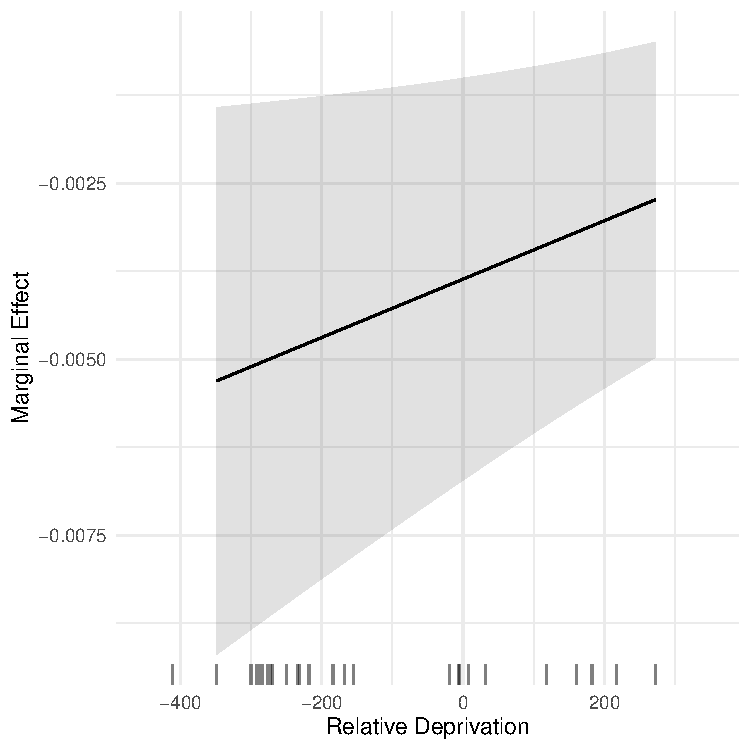
\includegraphics[width=1\textwidth]{figures/me_lpm.pdf}
\end{figure}

\subsection{Diagnostics}

Some diagnostics were conducted to see whether the LPM functional form is suitable for the outcome variable of violent unrest. First, to test the validity of the model, the fitted values were checked. In the data, 46.22\% of values fall outside of the [0, 1] range, with fitted values falling within the [-.0091, .84] range. This is a substantial deviation, which indicates that an LPM might not be suitable for the data. As the validity of the model is low, other models should be taken into account and tested. The reason might be that violent events are rare; not all municipalities experience a violent event. LPM additionally imposes no bounds and instead fits the binary outcome linearly, which might not be adequate for rare events.

Second, a nested model comparison is used to see how the interaction differs across different model specifications. When using no fixed effects, the interaction is positive and significant, \textit{b} = 0.0000080, \textit{SE} = 0.0000022, \textit{t} = 2.45, \textit{p} = .014. The overall model fit is, similarly to the two-way fixed effects model, poor, although better, adjusted \textit{R}\textit{\textsuperscript{2}} = .0011. In total, the model explains 0.11\% of the variance in the outcome.

With only municipality fixed effects, the interaction remains positive and significant, \textit{b} = 0.0000040, \textit{SE} = 0.0000016, \textit{t} = 2.45, \textit{p} = .014. The R\textsuperscript{2}, however, increases, adjusted \textit{R}\textit{\textsuperscript{2}} = .22. This means that the model with the municipal fixed effects explains 22.40\% of the variance. With only time fixed effects, the interaction is still positive and significant, \textit{b} = 0.000010, \textit{SE} = 0.0000029, \textit{t} = 3.49, \textit{p} < .001. The model explains little variance—0.39\%—in the outcome, adjusted \textit{R}\textit{\textsuperscript{2}} = .0039.

Given the results of the comparison, it can be concluded that cross-sectional heterogeneity between the municipalities explains the most variance in the outcome. However, the direction of the finding remained the same across models as well as significant. This shows that although the fixed effects drive most of the relationship, the core findings remain the same across models. All of them remain directionally the same as well as statistically significant.

Finally, to check whether a spatial model should be preferred, Moran’s I was assessed. The results show that Moran’s I was significant, \textit{I} =.12, \textit{SD} = 14.92, \textit{p} < .001. This means that the model’s residuals are spatially clustered, indicating that a spatial model would have been more appropriate. The standard errors of the LPM model are only clustered by municipality, which means that spatial spillovers between municipalities are not accounted for. This poses a noteworthy limitation which should have been accounted for.

\subsection{Robustness}

As a robustness check, a Poisson regression model was run to test the relationship between CCT payments and violent unrest in Brazil. To interpret the results, the coefficients were exponentiated in order to determine the respective incidence rate ratio (IRR). In the baseline model, the relationship was shown to be negative and non-significant, \textit{b} = -0.035, \textit{SE} = 0.20, \textit{z} = -0.18, \textit{p} = .86. The log-transformed payments showed an IRR of .97, which, given non-significant results, cannot be interpreted substantially.

In the interaction model, log-transformed CCT payments were shown to be negatively and non-significantly related to violent unrest, \textit{b} = -0.048, \textit{SE} = 0.22, \textit{z} = -0.21, \textit{p} = .83. Relative deprivation was shown to be positive and non-significant, \textit{b} = 0.00039, \textit{SE} = 0.0011, \textit{z} = 0.35, \textit{p} = .72. The interaction between CCT payments and relative deprivation was negative and non-significant, \textit{b} = -0.000071, \textit{SE} = 0.00019, \textit{z} = -0.37, \textit{p} = .71. The IRR was calculated to lie at .95 for the interaction model, though again, it cannot be interpreted given the non-significant results.

As both models were non-significant, none of the coefficients can be interpreted substantially. In sum, no effect on violent unrest could be established. Note that in both models, the observations dropped to 96,030, as the Poisson regression models dropped all municipalities that had no variation across all periods that were observed. This reduced the total number of observations significantly. Table 3 reports the results, and Figure 2 shows the marginal effects of the interaction model.

\begin{table}
\caption{Poisson Regression Model Results}
\centering
\begin{talltblr}[         %% tabularray outer open
entry=none,label=none,
note{}={+ p \num{< 0.1}, * p \num{< 0.05}, ** p \num{< 0.01}, *** p \num{< 0.001}},
]                     %% tabularray outer close
{                     %% tabularray inner open
colspec={Q[]Q[]Q[]},
hline{2}={1-3}{solid, black, 0.05em},
hline{8}={1-3}{solid, black, 0.05em},
hline{1}={1-3}{solid, black, 0.08em},
hline{18}={1-3}{solid, black, 0.08em},
column{2-3}={}{halign=c},
column{1}={}{halign=l},
}                     %% tabularray inner close
& Baseline & Interaction \\
log\_payment & \num{-0.035} & \num{-0.048} \\
& (\num{0.199}) & (\num{0.224}) \\
rel\_deprivation &  & \num{0.000} \\
&  & (\num{0.001}) \\
log\_payment × rel\_deprivation &  & \num{-0.000} \\
&  & (\num{0.000}) \\
Num.Obs. & \num{96030} & \num{96030} \\
R2 & \num{0.419} & \num{0.419} \\
R2 Adj. & \num{0.376} & \num{0.376} \\
R2 Within & \num{0.000} & \num{0.000} \\
R2 Within Adj. & \num{-0.000} & \num{-0.000} \\
AIC & \num{30435.1} & \num{30438.6} \\
BIC & \num{40362.2} & \num{40384.6} \\
RMSE & \num{0.31} & \num{0.31} \\
FE: muni\_norm & X & X \\
FE: time\_id & X & X \\
\end{talltblr}
\end{table}


\begin{figure}
    \centering
    \caption{Poisson Regression Model Interaction Effect}
    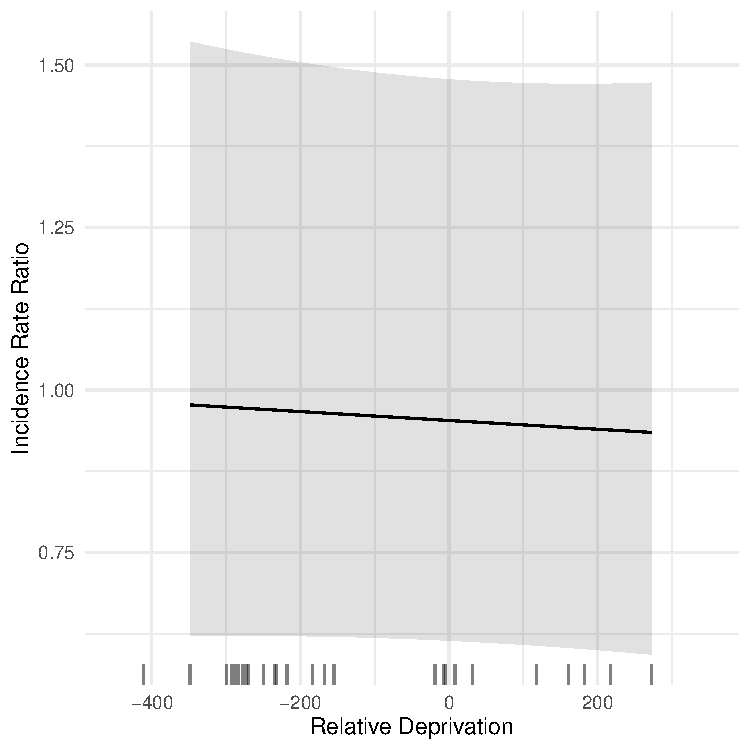
\includegraphics[width=1\textwidth]{figures/me_poisson.pdf}
\end{figure}

\section{Discussion}

In this section, the results will be discussed. First, depending on the model, H\textsubscript{1} and H\textsubscript{2} could or could not be supported. H\textsubscript{1} hypothesised that there is a negative link between CCT payments and violent unrest in Brazil, while H\textsubscript{2} hypothesised that higher levels of relative deprivation, proxied through income inequality, would weaken the relationship between payments and violence. The LPM model showed statistical significance and supported the directionality of the hypotheses, which could lead to the acceptance of the hypotheses. However, the diagnostics as well as the robustness check make it apparent that the initial LPM model might be unsuitable.

For one, the fitted values fall largely outside of the range, which is a threat to the validity of the model. In addition to that, the results of the nested comparison show that the interaction effect decreases once the municipality fixed effects are added to the models. This may indicate that the relationship might have been primarily driven by the fixed effects in the LPM model rather than the predictor. This poses a threat to the model worthy of being made explicit. Although the directionality was upheld throughout the different models, the small within R\textsuperscript{2} as well as the changes when adding the fixed effects should be considered.

This is further emphasised by the results of the Poisson regression models. They showed that the relationship between CCT payments and violent unrest, as well as the interaction effect, was non-significant. Additionally, the directionality of the interaction changed: Rather than dampening the relationship, relative deprivation exacerbates it. That is to say that the results of the LPM model did not hold up in the robustness check, which further implies that the model was not adequate to test the relationship.

Additionally, the results of the Moran’s I test indicate that a spatial panel model would have been preferred. The results, however, may have been sensitive to the distance. The diagnostics used a fixed number of nearest neighbours (\textit{k} = 5), but sparsity differs depending on the state of Brazil. Around the coast, the municipalities are much more dense and clustered together than in the interior of the country. As such, the spatial weights might not accurately consider the relationships with neighbouring municipalities across the country.

In sum, the LPM failed to meet the requirements set by the diagnostic tests. In other words, it was found to be inadequate. Additionally, it did not show any significance in the Poisson regression model. As such, the relationship could not be established. A possible explanation is that there is simply no relationship between CCT payments and violent unrest. Given previous literature on the subject matter, however, it seems quite unlikely that there is no connection between the two, as there has been research both showing that cash transfers might increase or reduce violence—them being unrelated seems not to be reported \parencite{machadoConditionalCashTransfer2018, zizumbo-colungaUnintendedConsequencesConditional2023}. Rather than a conceptual issue, this could be a methodological one, meaning that the operationalisation failed. Further research should investigate as to whether this is the case.

In addition, the mechanism could not be adequately tested. Possibly, relative deprivation as measured through income inequality is not a moderator of the relationship. Previous research used relative deprivation as a mediating rather than moderating variable \parencite{jiangRelativeDeprivationMechanism2020}. Future research could test as to whether this is an actuality. Other mechanisms could be tested as well, such as absolute deprivation, which was considered in other previous research \parencite{burrastonRelativeAbsoluteDeprivations2018} .

Finally, as the municipality fixed effects seem to be the main driver of the relationship, it would be sensible if future research uses other approaches to see whether the results are upheld. For instance, in addition to using fixed effects, future research could use control variables to see how it would change the model fit, such as municipal gross domestic product, unemployment, public spending, and electoral results. This could perhaps be a better approach rather than using just fixed effects, as they may obscure the relationship.

In sum, this research note constitutes a provocation about research gaps on the effect of CCT programmes with regard to spillover effects in novel areas. Further inquiry is necessitated as to whether the relationship is truly present, as well as whether deprivation constitutes a sensible explanatory mechanism. As such, further investigation is required to determine this association. Different modelling approaches are recommended.

\section{Conclusion}

In conclusion, this research note tested the relationship between CCT payments and violent unrest in Brazil, using income inequality as a moderator. Although the LPM model showed statistical significance, a small within R\textsuperscript{2}, as well as diagnostics, flag that the results must be looked upon with a sceptical eye. In addition, the Poisson regression model, which was run as a robustness check, yielded non-significant results and reversed the directionality of the interaction. As such, the relationship between the variables cannot be established in this research note. The proposed mechanism could also not be confirmed. Future research should attempt different identification strategies and operationalisation to further test whether an effect is present.

\printbibliography

\end{document}
